%----------------------------------------------------------------------------
\chapter{A vizualizálni kívánt rendszer bemutatása}
\label{chapt:birdnetes-introduction}
%----------------------------------------------------------------------------
Az alkalmazásom célja egy létező rendszer, a Birbnetes folyamatainak vizualizálása.
Ebben a fejezetben ismertetem a Birbnetes mikroszolgáltatás rendszerének architektúráját és az általa használt technológiákat.
Részletesen kifejtem az alkalmazásom szempontjából fontos komponensek feladatát és működését.

%----------------------------------------------------------------------------
\section{Elméleti összefoglaló}
%----------------------------------------------------------------------------
A bemutatásra kerülő rendszert a tanszéken egy projekt keretén belül készítették kollégáim,
melyet részletesen dokumentálták korábbi nyilvános publikációkban \cite{birdnetes-tdk} \cite{birdnetes-thesis}.
A következőkben a rendszer által használt technológiákat és elveket csak olyan szinten részletezem,
hogy annak működése érhető legyen.

%----------------------------------------------------------------------------
\subsection{Cloud, felhőalapú rendszerek}
%----------------------------------------------------------------------------
A cloud lényegében annyit jelent, hogy a szervert, amin az alkalmazás fut, nem a fejlesztőnek kell üzemeltetnie,
hanem valamilyen másik szervezet\footnotemark által vannak karban tartva. 
Ez több okból is hasznos:
\begin{itemize}
    \item \textbf{Költséghatékonyabb}. Nem szükséges berendezéseket vásárolni, azok üzemeltetési díja nem közvetlen a fejlesztőt éri. Az egyetlen költség a bérlés, ami általában töredéke annak, amit akkor fizetnénk ha magunk csinálnánk az egészet.
    \item \textbf{Gyorsabb fejlesztés}. Az alkalmazás futtatására használt szervereket általában a fejlesztő nem látja, ezekkel nem kell foglalkoznia. Ha az alkalmazásnak hirtelen nagyobb erőforrás igénye lesz, a rendszer automatikusan skálázódik.
    \item \textbf{Nagyobb megbízhatóság}. Az ilyen szolgáltatást nyújtó szervezeteknek ez az egyik legnagyobb feladata. Az alkalmazás bárhol és bármikor elérhető.
\end{itemize}

\footnotetext{Ilyenek például a Microsoft Azure, az Amazon Web Services vagy a Google Cloud.}
%----------------------------------------------------------------------------
\subsubsection{Mikroszolgáltatások}
%----------------------------------------------------------------------------
A mikroszolgáltatások (microservices) nem sok mindenben különböznek egy általános szolgáltatástól. 
Ugyan úgy valamilyen kéréseket kiszolgáló egységek, legyen az web kérések kiszolgálása HTTP-n keresztül
vagy akár parancssori utasítások feldolgozása. Az egyetlen fő különbség az a szolgáltatások felelősségköre.
A mikroszolgáltatások fejlesztésénél a fejlesztők elsősorban arra törekednek, hogy egy komponensnek minél kevesebb feladata és függősége legyen, 
ezzel megnő a tesztelhetőség és könnyebb a skálázhatóság.

%----------------------------------------------------------------------------
\subsubsection{Konténerek}
%----------------------------------------------------------------------------
A konténerek az operációs rendszer virtualizációt megvalósító egyik alkalmazása. 
Ezekre különböző korlátozások rakhatók például, hogy a konténer nem látja a teljes fájlrendszert, annak csak egy kijelölt részét,
megadható a konténer által használható processzor és memória igény vagy akár korlátozható az is, hogy a konténer hogyan használhatja a hálózatot.
Léteznek eszközök, például a Docker \cite{docker}, mely lehetővé teszi a fejlesztők számára az ilyen konténerek könnyed létrehozását és futtatását.

%----------------------------------------------------------------------------
\subsubsection{Kubernetes}
%----------------------------------------------------------------------------
A Kubernetes \cite{kubernetes} a komplex konténerizált mikroszolgáltatás rendszerek menedzselésének könnyítését szolgálja.
Kihasználja és ötvözi az imént említett technológiák előnyeit, hogy egy robosztus rendszert alkosson. 
Használatával felgyorsulhat és automatizált lehet az egyes konténerek telepítése, futtatása, de talán a legfőbb előnye,
hogy segítségével könnyedén megoldható a rendszert ért terhelési igények szerinti dinamikus skálázódás. 
Azok a mikroszolgáltatások, amikre a rendszernek épp nincs szüksége, minimális erőforrást igényelnek a szerveren,
így nem kell utánuk annyit fizetni sem. Ezzel ellentétben, ha valamely szolgáltatás után hirtelen megnő az igény,
akkor az könnyedén duplikálható.

%----------------------------------------------------------------------------
\subsection{MQTT}
\label{subsect:mqtt}
%----------------------------------------------------------------------------
Az MQTT (Message Queue Telemetry Transport) az egy kliens-szerver publish/subscribe üzenetküldő protokoll. Könnyű implementálni és alacsony a sávszélesség igénye,
mellyel tökéletes jelöltje a Machine to Machine (M2M), illetve az Internet of Things (IoT) kommunikáció megvalósítására.
Működéséhez szükség van egy szerverre, amelynek feladata a beérkező üzenetek tovább küldése témák alapján. Egyes kliensek fel tudnak iratkozni bizonyos témákra, míg más kliensek publikálnak
és a szerver levezényli a két fél között a kommunikációt.

%----------------------------------------------------------------------------
\subsection{OpenAPI}
%----------------------------------------------------------------------------
Az OpenAPI egy nyilvános alkalmazás-programozási leíró, amely a fejlesztők számára hozzáférést biztosít egy másik alkalmazáshoz.
Az API-k leírják és meghatározzák, hogy egy alkalmazás hogyan kommunikálhat egy másikkal, 
melyet használva a fejlesztők könnyedén képesek a kommunikációra képes kódot írni vagy generálni.

%----------------------------------------------------------------------------
\section{Rendszerszintű architektúra}
%----------------------------------------------------------------------------
A Birbnetes fejlesztése során kifejezetten fontos szerepe volt a mikroszolgáltatás alapú rendszerek elvei követésének.
A rendszer egy Kubernetes klaszterben van telepítve és több kisebb komponensből áll, melyek egymás között a HTTP és az MQTT protokollok segítségével kommunikálnak.
A rendszer összes szolgáltatásának van egy OpenAPI leírója, melyet használva hamar volt egy olyan kódbázisom, amely képes volt a rendszerrel való kommunikációra.


%----------------------------------------------------------------------------
\subsection{Főbb komponensek}
%----------------------------------------------------------------------------
A \ref{fig:birdnetes-components}-es ábrán láthatóak a rendszer komponensei, melyek mindegyike egy-egy mikroszolgáltatás.
Az egymás mellett lévő kék levélborítékok az MQTT kommunikációt jelölik,
amellyel például a természetben elhelyezett eszközök felé irányuló kommunikáció is történik.
A következő alszakaszokban bemutatom az alkalmazásom szempontjából fontosabb komponenseket.

\begin{figure}[!ht]
\centering
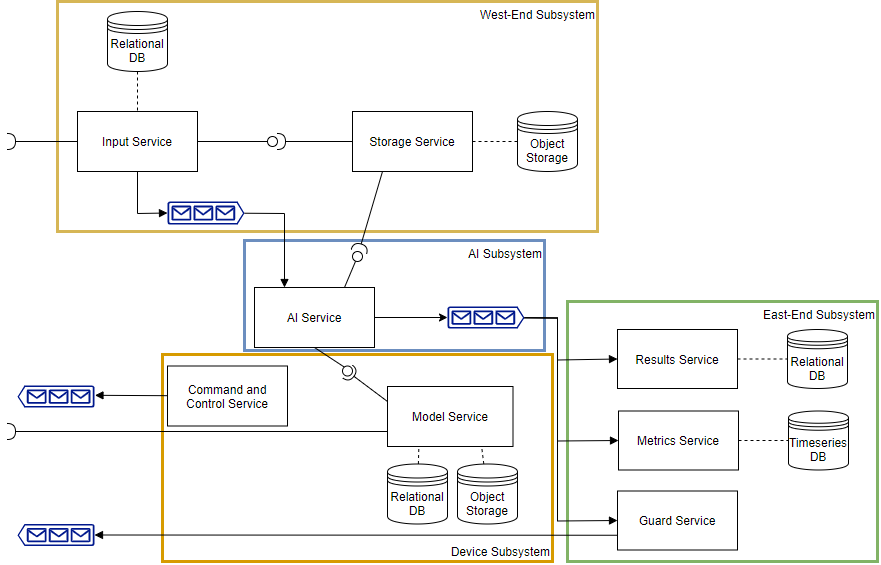
\includegraphics[width=150mm, keepaspectratio]{figures/architecture-redesigned.png}
\caption{A Birbnetes rendszer architektúrája. Forrás: Madárhang azonosító és riasztó felhő-natív rendszer TDK dolgozat \cite{birdnetes-tdk}}
\label{fig:birdnetes-components}
\end{figure}

%----------------------------------------------------------------------------
\subsubsection{IoT eszközök}
%----------------------------------------------------------------------------
Szőlőültetvényekben telepített eszközök, melyek adott időközönként publikálják állapotaikat egyéb metaadatokkal egy üzenetsoron.
Emellett folyamatosan hangfelvételt készítenek a beépített mikrofonjaikkal, mely hangfelvételekről egy másik belső szenzor eldönti,
hogy érdemes-e felküldeni a rendszerbe, ha igen, akkor egy másik üzenetsoron publikálják ezeket a hangfelvételeket.
Tartalmaznak még egy hangszórót is, mely a madarak elijesztését szolgálja.

%----------------------------------------------------------------------------
\subsubsection{Input Service}
\label{subsect:birdnetes-input-service}
%----------------------------------------------------------------------------
A kihelyezett IoT eszközök által felvett hangfájlok ezen a komponensen keresztül érkeznek be a rendszerbe.
Itt történik a hanganyaghoz tartozó metaadatok lementése az Input Service saját relációs adatbázisába. 
Ilyenek például a beküldő eszköz azonosítója, a beérkezés dátuma vagy a hangüzenet rendszerszintű egyedi azonosítója.
Amint a szolgáltatás a beérkezett üzenettel kapcsolatban elvégezte az összes feladatát, 
publikál egy üzenetet egy másik üzenetsorra a többi kliensnek feldolgozásra.

%----------------------------------------------------------------------------
\subsubsection{AI Service}
\label{subsect:birdnetes-ai-service}
%----------------------------------------------------------------------------
Az AI Service példányai fogadják az Input Service-től érkező üzeneteket és elkezdik klasszifikálni az abban található hanganyagot.
Meghatározzák, hogy a hanganyag mekkora valószínűséggel volt seregély hang vagy sem.
Ennek eredményét a hangminta egyedi azonosítójával együtt publikálják egy másik üzenetsoron.

%----------------------------------------------------------------------------
\subsubsection{Guard Service}
%----------------------------------------------------------------------------
A Guard Service feliratkozik az AI Service által publikált üzenetek témájára 
és valamilyen valószínűségi kritérium alapján eldönti, hogy a hangminta tartalmaz-e seregély hangot.
Ha igen, akkor az üzenetsoron küld egy riasztás parancsot a hanganyagot küldő eszköznek.

%----------------------------------------------------------------------------
\subsubsection{Command and Control Service}
%----------------------------------------------------------------------------
A Command and Control Service az előzőkkel ellentétben egyáltalán nem vesz részt a minták fogadásában, feldolgozásában vagy kezelésében.
Felelősége az eszközök és azok szenzorjai állapotának menedzselése és követése.
Ezen keresztül lehet az egyes eszközöket ki- és bekapcsolni.